\section{Auswertung}
\label{sec:Auswertung}
  \subsection{Winkelrichtgröße und Eigenträgheitsmoment}







\begin{figure}
  \centering
  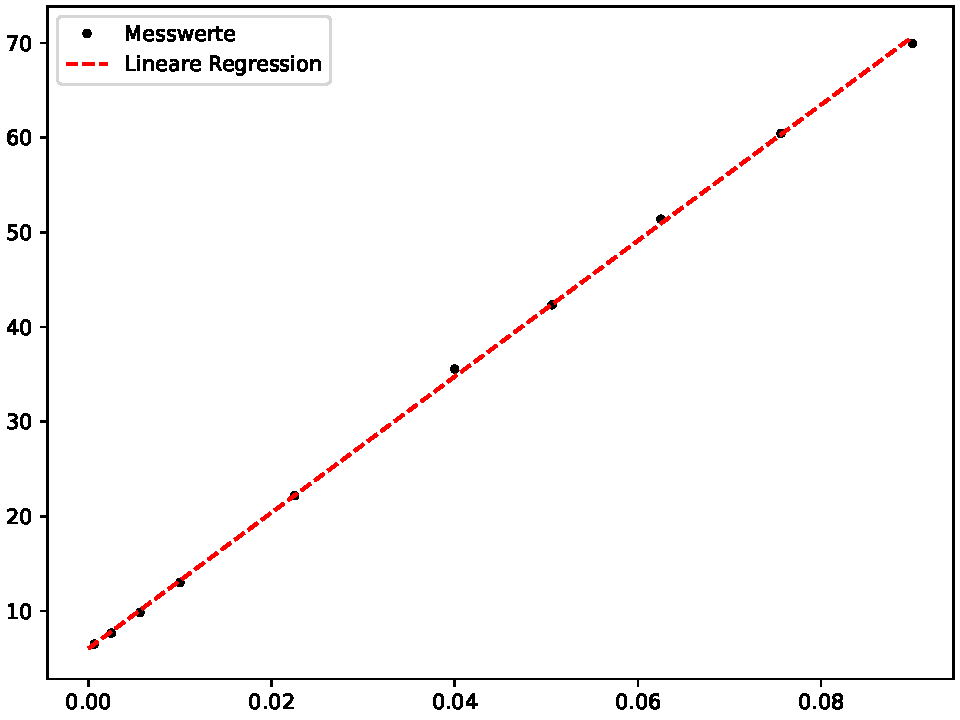
\includegraphics{plot.pdf}
  \caption{Plot.}
  \label{fig:plot}
\end{figure}

\begin{table}
  \centering
  \caption{Tabelle 1}
  \label{tab:tabelle}
  \sisetup{table-format=1.1, per-mode=reciprocal}
  \begin{tblr}{
      colspec = {S[table-format=3.0] S[table-format=2.1] S},
      row{1} = {guard, mode=math},
      vline{4} = {2}{-}{text=\clap{$\pm$}},
    }
    \toprule
    F \mathbin{/} \unit{\newton} & $\varphi$ \mathbin{/} \unit{\degree} & \SetCell[c=2]{c} $\symbf{D}$ \mathbin{/} \unit{\newton\meter} & \\
    \midrule
    0.016&   20   & 0.009\\
    0.046&   30   & 0.018\\
    0.066&   40   & 0.019\\
    0.089&   50   & 0.020\\ 
    0.11 &   60   & 0.021\\
    0.134&   70   & 0.022\\
    0.162&   80   & 0.023\\
    0.176&   90   & 0.022\\
    0.18 &  100   & 0.021\\
    0.2  &  110   & 0.021\\
    0.23 &  120   & 0.022\\
    \bottomrule
  \end{tblr}
\end{table}

Siehe \autoref{fig:plot} und \autoref{tab:tabelle}!
